\section{Aufgabe 3}
Prinzipiell ist das Vorgehen bei der Ausführung identisch zu dem in Aufgabe 2. Bei der Auswertung ist jedoch nicht der Plattenabstand \(d\) sondern die Wellenlänge \(\lambda \) gesucht, die Formel \eqref{b} wird daher nach \(\lambda \) aufgelöst. Alexander Heinisch nahm die Messung mit blauen Filter vor, Dominik Wille die mit dem grünen Filter.
\subsection{Fehlerabschätzung}
Identisch zu Aufgabe 2 wird der Fehler des Radius' bestimmt aus
\begin{align}
\Delta r &= \frac{1}{2} \cdot \sqrt{
\left( \frac{x_{i,links} - x_{a,links}}{2} \right)^2 +
\left( \frac{x_{i,rechts} - x_{a,rechts}}{2} \right)^2
} \notag
\end{align}
\begin{align}
\Delta \left( r_0^2 - r_j^2 \right) &= \sqrt{
\left( 2 r_0 \cdot \Delta r_0 \right)^2 +
\left( 2 r_j \cdot \Delta r_j \right)^2
} \notag
\end{align}
\subsection{Gegebenes}
Um die Wellenlänge in dieser Aufgabe zu bestimmen, wird der ermittelte Plattenabstand \(d\) aus Aufgabe 2 verwendet. Die Gegeben Daten sind daher:
\begin{center}
\begin{tabular}{rcc}
\(d\) & \(=\) & \(\left( 3,66 \pm 0,16 \right)\, mm\) \\
\(f\) & \(=\) & \(\left( 10,0 \pm 0,5 \right)\, cm\) \\
\end{tabular}
\end{center}
\subsection{Beobachtung}
Qualitativ zeigte das Bild sowohl beim blauen als auch beim grünen Glas wieder Kreise in der Farbe des Filters, also in diesem Fall blau oder grün. Quantitativ waren die Kreise jedoch kleiner als bei dem roten Filter. Die blauen Kreise waren dabei am kleinsten. Da evtl. beim Grünen Farbglas ein Messwert (Messwert bei n = 3) übersehen werden auch die verschobenen Messwerte ausgewertet.
\subsection{Messwerte und Graphen}
\begin{center}
\begin{tabular}{c|ccc|ccc|c|c} 
Ordnung \(n\) & \multicolumn{3}{c|}{\(x_{i,links}\)} & \multicolumn{3}{c|}{\(x_{i,rechts}\)} & \(r\) & \(\left( r_i^2 - r_0^2 \right)\)\\
& \multicolumn{3}{c|}{\(mm\)} & \multicolumn{3}{c|}{\(mm\)}  & \(mm\) & \(mm^2\) \\ \hline
\(1\) & N/A & - & \(9,90\) & N/A & - & \(11,59\) & \(0,085\) & \\ 
\(2\) & \(9,61\) & - & \(9,35\) & \(11,78\)  & - & \(12,10\) & \(1,23\pm 0,10\) & \(0,00\pm 0,36\)\\ 
\(3\) & \(9,18\) & - & \(8,96\) & \(12,25\)  & - & \(12,49\) & \(1,650\pm 0,081\) & \(1,21\pm 0,37\)\\ 
\(4\) & \(8,86\) & - & \(8,63\) & \(12,58\)  & - & \(12,81\) & \(1,975\pm 0,081\) & \(2,39\pm 0,41\)\\ 
\(5\) & \(8,49\) & - & \(8,32\) & \(12,91\)  & - & \(13,15\) & \(2,313\pm 0,074\) & \(3,83\pm 0,42\)\\ 
\(6\) & \(8,18\) & - & \(8,04\) & \(13,25\)  & - & \(13,41\) & \(2,610\pm 0,053\) & \(5,30\pm 0,38\)\\ 
\(7\) & \(7,92\) & - & \(7,81\) & \(13,52\)  & - & \(13,78\) & \(2,893\pm 0,070\) & \(6,85\pm 0,48\)\\ 
\(8\) & \(7,71\) & - & \(7,54\) & \(13,79\)  & - & \(14,00\) & \(3,135\pm 0,068\) & \(8,32\pm 0,49\)\\ 
\(9\) & \(7,43\) & - & \(7,33\) & \(14,15\)  & - & \(14,27\) & \(3,415\pm 0,039\) & \(10,15\pm 0,37\)\\ 
\(10\) & \(7,25\) & - & \(7,18\) & \(14,39\)  & - & \(14,47\) & \(3,608\pm 0,027\) & \(11,50\pm 0,32\)\\ 

\end{tabular}
{\it Tab. 3.1: Messwerte für das blaue Farbglas Phywe (8402)}
\vspace{5mm}
\\
\begin{tabular}{c|ccc|ccc|c|c} 
Ordnung \(n\) & \multicolumn{3}{c|}{\(x_{i,links}\)} & \multicolumn{3}{c|}{\(x_{i,rechts}\)} & \(r\) & \(\left( r_i^2 - r_0^2 \right)\)\\
%& i & a & i & a \\
& \multicolumn{3}{c|}{\(mm\)} & \multicolumn{3}{c|}{\(mm\)}  & \(mm\) & \(mm^2\) \\ \hline
\(1\) & \(10.3\) & - & \(9.81\) & \(11.07\) & - & \(11.5\) & \(0.615\) & \\ 						
\(2\) & \(9.52\) & - & \(9.31\) & \(11.94\) & - & \(12.12\) & \(1.308\pm 0.070\) & \(0.00\pm 0.26\)\\
\(3\) & \(9.02\) & - & \(8.82\) & \(12.35\) & - & \(12.53\) & \(1.760\pm 0.068\) & \(1.39\pm 0.30\)\\
\(4\) & \(8.70\) & - & \(8.56\) & \(12.77\) & - & \(12.86\) & \(2.093\pm 0.042\) & \(2.67\pm 0.26\)\\
\(5\) & \(8.38\) & - & \(8.28\) & \(13.50\) & - & \(14.16\) & \(2.750\pm 0.170\) & \(5.86\pm 0.94\)\\
\(6\) & \(8.10\) & - & \(7.95\) & \(14.33\) & - & \(14.43\) & \(3.178\pm 0.046\) & \(8.39\pm 0.34\)\\
\(7\) & \(7.74\) & - & \(7.21\) & \(14.56\) & - & \(14.65\) & \(3.565\pm 0.140\) & \(11.00\pm 0.98\)\\
\(8\) & \(7.58\) & - & \(7.52\) & \(14.70\) & - & \(14.77\) & \(3.593\pm 0.024\) & \(11.20\pm 0.25\)\\
\(9\) & \(7.43\) & - & \(7.31\) & \(15.02\) & - & \(15.10\) & \(3.845\pm 0.037\) & \(13.08\pm 0.34\)\\
\(10\) & \(7.22\) & - & \(7.17\) & \(15.20\) & - & \(15.29\) & \(4.025\pm 0.026\) & \(14.50\pm 0.28\)\\
\end{tabular}
{\it Tab. 3.2: Messwerte für das grüne Farbglas Phywe (8404)}
\\
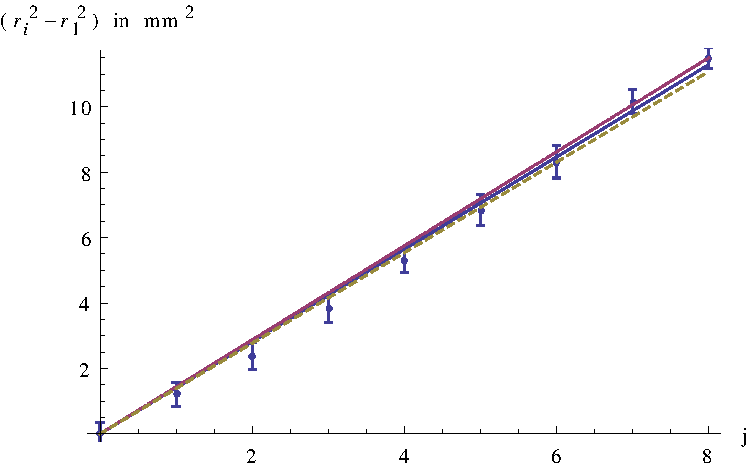
\includegraphics[width=12cm]{graphen/blau}
{\it Abbildung. 3.1: Messwerte mit blauen Farbglas Phywe (8402) aufgetragen über \(j\)}
\\
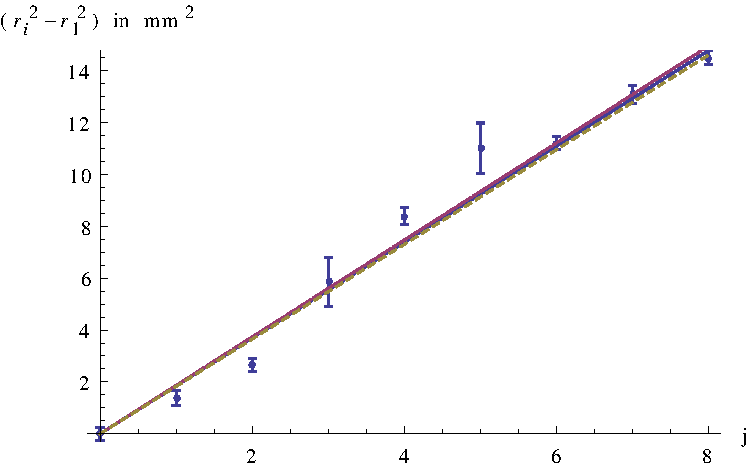
\includegraphics[width=12cm]{graphen/gruen}
{\it Abbildung. 3.2: Messwerte mit grünem Farbglas Phywe (8404) aufgetragen über \(j\)}
\\
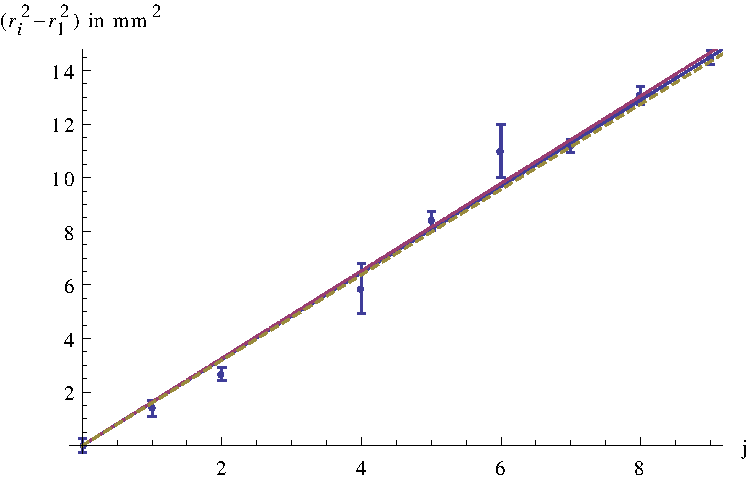
\includegraphics[width=12cm]{graphen/gruen_new}
{\it Abbildung. 3.3: verschobene Messwerte mit grünem Farbglas Phywe (8404) aufgetragen über \(j\)}

\end{center}
Die Steigungen \(b\) wurde mittels linearer Regression bestimmt zu:
\begin{align}
b_{blau} &= \left( 1,411 \pm 0,026 \right)\,mm^2 \notag\\
b_{grün} &= \left( 1,846 \pm 0,022 \right)\,mm^2 \notag\\
b_{grün_{verschoben}} &= \left( 1,612 \pm 0,019 \right)\,mm^2 \notag
\end{align}
\subsection{Auswertung}
Um die Wellenlänge aus den gemessenen Daten bestimmen zu können, wird Gleichung \eqref{b} nach \(\lambda\) aufgelöst. Das ergibt:
\begin{equation}
\lambda = \frac{bd}{f^2} \notag
\end{equation}
Für den Fehler folgt daraus:
\begin{align}
\Delta \lambda &= \sqrt{
\left( \frac{\partial \lambda}{\partial b} \cdot \Delta b \right)^2 +
\left( \frac{\partial \lambda}{\partial f} \cdot \Delta f \right)^2
} \notag \\
&= \lambda \cdot \sqrt{
\left( \frac{\Delta b}{b} \right)^2 +
\left( \frac{2 \Delta f}{f}\right)^2
} \notag
\end{align}
Ausgerechnet ergibt das:
\begin{align}
\lambda_{blau} &= \left( 516 \pm 13 \right)\, nm \notag \\
\lambda_{grün} &= \left( 676 \pm 15 \right)\, nm \notag \\
\lambda_{grün_{verschoben}} &= \left( 590 \pm 14 \right)\, nm \notag
\end{align}

Zum Vergleich gilt für die Literaturwerte:
\begin{center}
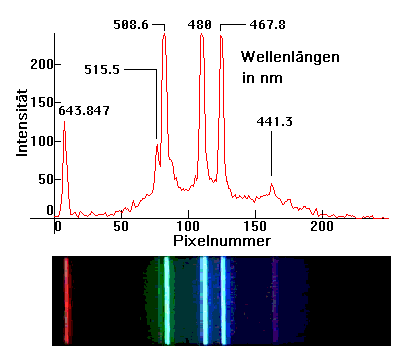
\includegraphics[width=8cm]{bilder/IMG_0020}

{\it Abbildung. 3.3: Darstellung der Hauptmaxima einer Cadmium-Lampe}
\end{center}

\newpage
\subsection{Fazit}
\begin{align}
\lambda_{blau} &= \left( 520 \pm 20 \right)\, nm \notag \\
\lambda_{grün} &= \left( 680 \pm 20 \right)\, nm \notag \\
\lambda_{grün} &= \left( 590 \pm 20 \right)\, nm \notag
\end{align}
\begin{center}
\it Endergebnis für \(\lambda_{blau}\) und \(\lambda_{grün}\)
\end{center}
Im Endergebnis wird klar, dass die Linien nicht zuordbar sind. Das hat verschiedene Ursachen. Zum einen ist die Messung des Plattenabstands \(d\) zu ungenau gewesen um eindeutige Zuordnungen zu gewährleisten, zum anderen sind die Ergebnisse nicht plausibel. Ein Grüner Filter sollte Emissionslinien mit kürzeren Wellenlängen passieren lassen als der rote Filter, die Ermittelte Wellenlänge beim grünen Filter ist aber länger. Und auch die mit dem blauen Filter ermittelte Wellenlänge passt nicht ins blaue Spektrum des sichtbaren Lichts. Die verschobenen Messwerte beim grünen Filter liefern auch kein akzeptables Ergebnis. Die Wellenlänge kann weder zugeordnet werden noch passt sie ins grüne Farbspektrum des sichtbaren Lichts

Zu sehen ist auch, dass Dominik Wille offensichtlich deutlich schlechter abgelesen hat als Alexander Heinisch, denn die Streuung der Messwerte ist beim grünen Filter am größten.
